\section{}

% A 3 m × 2 m thin rectangular plate is deformed by the movement of point B to B′ as shown by the
% dashed lines in Fig. 2. Assuming a displacement field of the form u = c1xy and v = c2xy where c1
% and c2 are constants, determine,
% (a) expressions for displacements u and v.
% (b) strain components εx, εy, and γxy at point B.
% (c) the normal strain εx′ in the direction of QB.
% Verify that the strain field is possible.

A $\qty{3}{\meter} \times \qty{2}{\meter}$ thin rectangular plate is deformed by the movement of point $B$ to $B'$ as shown by the dashed lines 
in Fig. \ref{fig:Q2}. Assuming a displacement field of the form $u = c_1xy$ and $v = c_2xy$ where $c_1$ and $c_2$ are constants, determine,

\begin{enumerate}[label=(\alph*)]
    \item Expressions for displacements $u$ and $v$.
    \item Strain components $\epsilon_x$, $\epsilon_y$, and $\gamma_{xy}$ at point $B$.
    \item The normal strain $\epsilon_{x'}$ in the direction of $\overline{QB}$.
\end{enumerate}


\begin{figure}[h]
    \centering
    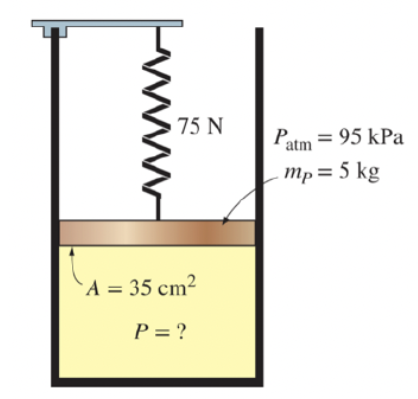
\includegraphics[width=0.5\linewidth]{Questions/Figures/Q2ProblemDiagram.png}
    \caption{Stress distribution on a thin rectangular plate.}
    \label{fig:Q2}
\end{figure}

\subsection{}
Using the geometry of the problem, the constants $c_1$ and $c_2$ can be determined. First, $c_1$:
\begin{align*}
    u &= c_1xy \\
    c_1 &= \frac{u}{xy} \\
    &= \frac{3}{2\times3\times 10^{6}} \\
    %&= 5\times10^{-7}
    &= \qty{5e-7}{\milli\meter^{-1}}
\end{align*}

Similarly, $c_2$ is given by:
\begin{align*}
    v &= c_2xy \\
    c_2 &= \frac{v}{xy} \\
    &= \frac{1.5}{2\times3\times 10^{6}} \\
    %&= 2.5\times10^{-7}
    &= \qty{2.5e-7}{\milli\meter^{-1}}
\end{align*}

Therefore the expressions for $u$ and $v$ are given by:
\begin{empheq}[box=\fbox]{align*}
    u &= 5\times10^{-7}xy \;\text{[mm]}\\
    v &= 2.5\times10^{-7}xy \;\text{[mm]}
\end{empheq}

\subsection{}
The strain components $\epsilon_x$, $\epsilon_y$, and $\gamma_{xy}$ at point $B$ are given by:
\begin{align*}
    \epsilon_x|_B &= \frac{\partial u}{\partial x}|_B = 5\times10^{-7}y|_B = 5 \times 10^{-7} \times 2000  = \boxed{\qty{1.00e-3}{}} \\
    \epsilon_y|_B &= \frac{\partial v}{\partial y}|_B = 2.5\times10^{-7}x|_B = 2.5 \times 10^{-7} \times 3000  = \boxed{\qty{7.50e-4}{}} \\
    \gamma_{xy}|_B &= \frac{\partial u}{\partial y} + \frac{\partial v}{\partial x}|_B = 5\times10^{-7}x+ 2.5\times10^{-7}y |_B \\
    &= 5\times10^{-7}\times3000+ 2.5\times10^{-7}\times2000 = \boxed{\qty{2.00e-3}{}}
\end{align*}

\subsection{}
Recall that the normal strain $\epsilon_{x'}$ in the direction of $\overline{QB}$ is given by:
\begin{equation*}
    \epsilon_{x'} = \epsilon_x\cos^2\theta + \epsilon_y\sin^2\theta + 2\gamma_{xy}\sin\theta\cos\theta
\end{equation*}

\begin{align*}
    \theta &= \tan^{-1}\left(\frac{\overline{BC}}{\overline{QC}}\right) \\
    &= \tan^{-1}\left(\frac{2000}{3000}\right) \\
    &= \ang{33.69} \\
\end{align*}

Therefore, by substitution,
\begin{align*}
    \epsilon_{x'} &= \epsilon_x\cos^2\theta + \epsilon_y\sin^2\theta + 2\gamma_{xy}\sin\theta\cos\theta \\
    &= \qty{1.00e-3}\cos^2(33.69) + \qty{7.50e-4}\sin^2(33.69) + 2\qty{2.00e-3}\sin(33.69)\cos(33.69) \\
    &= \boxed{\qty{1.85e-3}{}}
\end{align*}

\subsection{}
The relevant compatibility equation for field is given by:
\begin{align*}
    2 \frac{\partial^2 \epsilon_{xy}}{\partial x \partial y} &= \frac{\partial^2 \epsilon_{x}}{\partial y^2} + \frac{\partial^2 \epsilon_{y}}{\partial x^2} \\
\end{align*}

The left hand side evaluates to:
\begin{align*}
    \frac{\partial^2 \gamma_{xy}}{\partial x \partial y} &= \frac{\partial^2}{\partial x \partial y}(5\times10^{-7}x + 2.5\times10^{-7}y) \\
    &= 0
\end{align*}

The right hand side evaluates to:
\begin{align*}
    \frac{\partial^2 \epsilon_{x}}{\partial y^2} + \frac{\partial^2 \epsilon_{y}}{\partial x^2} &= \frac{\partial }{\partial y}(5\times 10^{-7}y) + \frac{\partial }{\partial x} (2.5\times 10^{-7}x) \\
    &= 0 + 0
\end{align*}

$\boxed{\text{Therefore, the compatibility equation is satisfied and the strain field is possible.}}$
